\documentclass[11pt,a4paper,twoside]{article}
\usepackage[utf8]{inputenc}
\usepackage[vietnamese]{babel}
\usepackage[T5]{fontenc}
\usepackage{amsmath,amssymb,amsfonts}
\usepackage{booktabs,longtable,multirow,tabularx}
\usepackage{graphicx,float,pdflscape}
\usepackage[font=small,labelfont=bf]{caption}
\usepackage{xcolor,hyperref,microtype,fancyhdr}
\usepackage[a4paper,left=27mm,right=27mm,top=23mm,bottom=25mm,headheight=16pt]{geometry}
\graphicspath{{figures/}}
\hypersetup{colorlinks=true,linkcolor=blue!55!black,citecolor=blue!55!black,urlcolor=blue!55!black}
\setlength{\parindent}{1.25em}
\setlength{\parskip}{0pt}
\sloppy
\pagestyle{fancy}
\fancyhf{}
\fancyhead[LE]{\small NHÓM NGHIÊN CỨU GSI-MLC-PA}
\fancyhead[RO]{\small SO SÁNH v6.3.3 VÀ v6.3.5}
\fancyfoot[C]{\thepage}
\renewcommand{\headrulewidth}{0pt}
\begin{document}
\thispagestyle{empty}
\noindent\small Báo cáo nghiên cứu thực nghiệm GSI-MLC-PA (2026) \hfill Hoàn thành 10/2026
\vspace{2.5em}
\begin{center}
{\LARGE\bfseries Phân loại đa nhãn với cơ chế từ chối theo cấu trúc nhãn:\\[0.25em] So sánh thực nghiệm BR, CC, MLC-PA, GSI-MLC-PA v6.3.3 và v6.3.5}\\[1.5em]
{\large\bfseries Nhóm nghiên cứu Machine Learning và Khai phá dữ liệu}\\[0.3em]
{\itshape Báo cáo nội bộ có khả năng tái lập; trình bày theo bố cục JAIR của Nguyen và Hüllermeier (2021)}\\
\end{center}
\vspace{1.2em}
\begin{center}\bfseries Tóm tắt\end{center}
Báo cáo đánh giá năm phương pháp phân loại đa nhãn trên mười tập dữ liệu bằng cùng một quy trình kiểm định chéo phân tầng 5-fold, cùng bộ phân loại Logistic Regression và cùng các fold. Hai mô hình BR và CC luôn dự đoán đầy đủ; MLC-PA sử dụng quyết định Bayes cho Hamming loss với chi phí từ chối $c=0.30$; GSI-MLC-PA v6.3.3 áp dụng suy diễn ba chế độ và từ chối trên mọi nhãn; v6.3.5 chỉ cho phép từ chối trên tập nhãn phụ thuộc DL, trong khi IL luôn trả quyết định. Kết quả cho thấy v6.3.3 đạt Selective Macro-F1 trung bình cao nhất (0.5759) ở coverage 0.7318. v6.3.5 tăng coverage lên 0.8212 nhưng Selective Macro-F1 giảm còn 0.5560. Dù vậy, v6.3.5 vẫn cao hơn đối chứng phi GSI tốt nhất (CC, 0.4796) về Selective Macro-F1. Kết quả được diễn giải như một đánh đổi coverage--chất lượng, không phải sự thống trị tuyệt đối của một mô hình.
\vspace{0.5em}
\noindent\textbf{Từ khóa:} phân loại đa nhãn; từ chối từng phần; selective prediction; Binary Relevance; Classifier Chains; GSI-MLC-PA.
\section{Giới thiệu}
Trong phân loại đa nhãn, một mẫu có thể đồng thời gắn với nhiều nhãn. Khi xác suất dự đoán không đủ tin cậy, partial abstention cho phép hệ thống chỉ từ chối một số vị trí nhãn thay vì từ chối toàn bộ mẫu. Khung quyết định này đặc biệt hữu ích khi chất lượng dự đoán và khối lượng cần chuyển cho con người cùng quan trọng \cite{nguyen2021,chow1970}. Tuy nhiên, F1 chọn lọc chỉ được tính trên các vị trí đã quyết định; vì thế mọi kết luận về F1 phải đi kèm coverage và chất lượng vùng bị từ chối.
Mục tiêu của báo cáo là kiểm định cơ chế v6.3.5: bỏ từ chối cho nhãn độc lập IL và chỉ giữ từ chối cho nhãn phụ thuộc DL. Báo cáo không sử dụng số liệu từ các runner cũ có cấu hình khác. Toàn bộ bảng và hình được sinh từ tệp \texttt{unified\_detailed\_folds.csv}, tạo bởi mã nguồn hiện tại ngày 14/10/2026.
\section{Các phương pháp so sánh}
\subsection{BR và CC}
Binary Relevance (BR) học một bộ phân loại nhị phân độc lập cho mỗi nhãn. Classifier Chains (CC) nối các nhãn theo thứ tự tự nhiên và dùng các dự đoán trước làm đặc trưng cho nhãn sau \cite{read2011}. Cả hai mô hình trong thực nghiệm này luôn xuất ma trận nhị phân đầy đủ, do đó coverage bằng 1.
\subsection{MLC-PA}
MLC-PA dùng xác suất biên từ BR và quy tắc Bayes tối ưu cho generalized Hamming loss dưới giả định độc lập nhãn \cite{nguyen2021}. Với phạt tuyến tính, mỗi lỗi đã quyết định có chi phí 1 và mỗi vị trí từ chối có chi phí $c=0.30$.
\subsection{GSI-MLC-PA v6.3.3 và v6.3.5}
v6.3.3 thực hiện peeling để chia nhãn thành IL/DL, dùng BR theo tầng cho IL, OS-NMF cho DL, hiệu chuẩn theo mất cân bằng và hai ngưỡng $\tau_0,\tau_1$ để quyết định 0, từ chối hoặc 1. Cấu hình thực tế dùng $c=0.30$, $\gamma_{min}=0.70$, $\tau_{balance}=0.85$, $\alpha=0.25$ và SAMG legacy.
v6.3.5 kế thừa SAMG2 OOF-guarded của v6.3.4. Sau khi tạo dự đoán chọn lọc, các ô IL đang từ chối được điền bằng quyết định đầy đủ theo ngưỡng thích ứng; cột DL không bị sửa. Vì vậy cơ chế mới trực tiếp tăng IL coverage lên 1, nhưng có thể đưa các trường hợp IL khó trở lại tập đánh giá.
\begin{table}[H]\centering
\caption{Tóm tắt cấu hình mô hình trong benchmark thống nhất.}
\label{tab:models}\small
\begin{tabularx}{\textwidth}{lXcc}\toprule
Mô hình & Cấu trúc & Có từ chối & Phạm vi từ chối \\\midrule
BR & Bộ phân loại nhị phân độc lập theo nhãn & Không & -- \\
CC & Chuỗi phân loại theo thứ tự nhãn tự nhiên & Không & -- \\
MLC-PA & BR xác suất + Hamming BOP, phạt tuyến tính & Có & Mọi nhãn \\
GSI v6.3.3 & Peeling IL/DL + OS-NMF + Tri-Regime + SAMG legacy & Có & Mọi nhãn \\
GSI v6.3.5 & v6.3.4/SAMG2 + quyết định đầy đủ cho IL & Có & Chỉ DL \\
\bottomrule\end{tabularx}\end{table}
\section{Thuật toán đề xuất: từ động cơ thiết kế đến triển khai}
\subsection{Bài toán mà thiết kế cần giải quyết}
Một ngưỡng $0.5$ chung cho mọi nhãn ngầm giả định rằng xác suất đã được hiệu chuẩn như nhau và hai lớp có mức độ khó tương đương. Giả định này không phù hợp với dữ liệu đa nhãn: prior của từng nhãn có thể chênh lệch lớn, một số nhãn còn dự đoán được từ đặc trưng đầu vào (IL), trong khi các nhãn khác vẫn chia sẻ sai số có cấu trúc (DL). Mặt khác, ép mô hình quyết định tại mọi vị trí làm các xác suất gần ranh giới trở thành lỗi; nhưng từ chối quá nhiều lại làm F1 chọn lọc tăng một cách không hữu dụng vì hệ thống chuyển phần lớn công việc cho khâu review. Do đó thuật toán phải đồng thời trả lời ba câu hỏi: xác suất được tạo ra thế nào, vị trí nào đủ tin cậy để quyết định, và nhóm nhãn nào thực sự được phép từ chối.
GSI-MLC-PA tách ba câu hỏi này thành ba tầng. Tầng cấu trúc phân chia IL/DL và chỉ mô hình hóa phụ thuộc khi còn bằng chứng trong phần dư. Tầng quyết định biến xác suất thành $0/-1/1$ bằng hai ngưỡng riêng cho từng nhãn. Tầng chính sách của v6.3.5 loại bỏ trạng thái $-1$ trên IL nhưng giữ nguyên nó trên DL. Sự tách biệt này là chủ ý: chi phí $c$ kiểm soát giá tương đối của việc từ chối, còn \texttt{rejection\_scope} kiểm soát nơi tổ chức cho phép từ chối; chúng không phải hai mô hình phân loại độc lập.
\subsection{Học cấu trúc nhãn và xác suất dự đoán}
Đầu tiên, CV peeling đánh giá từng nhãn bằng dự đoán out-of-fold (OOF). Nhãn đạt tiêu chuẩn ở một tầng được đưa vào IL; xác suất OOF của IL đã chọn được chuẩn hóa rồi nối vào $X$ để tầng sau có thể sử dụng thông tin đã học mà không nhìn nhãn thật của chính mẫu đó. Cách dùng OOF ở đây nhằm ngăn rò rỉ dữ liệu khi chọn cấu trúc. Các nhãn còn lại tạo thành DL. Mỗi DL có một mô hình BR nền trên không gian đặc trưng sau peeling.
Với ít nhất hai DL, chương trình tính phần dư giữa nhãn thật và xác suất OOF, sau đó tính tương quan Pearson có dấu giữa các cột phần dư. Chỉ các cạnh có độ lớn tương quan đạt $0.25$ mới được giữ. OS-NMF thực hiện đúng một bước hiệu chỉnh logit với hệ số $\alpha=0.25$, chuẩn hóa theo bậc và chặn dịch logit để tránh khuếch đại vòng lặp. Một bước là lựa chọn có chủ đích: nó khai thác tín hiệu phụ thuộc còn lại nhưng không biến suy diễn thành quá trình lặp khó ổn định. Sau đó bộ hiệu chuẩn thích nghi được fit trên xác suất OOF và áp dụng nhất quán cho xác suất huấn luyện/test.
\subsection{Từ chi phí $c$ đến hai ngưỡng thích nghi}
Nếu xác suất hậu nghiệm đã hiệu chuẩn là $p=P(y=1\mid x)$, chi phí dự đoán 0 là $p$, chi phí dự đoán 1 là $1-p$, còn chi phí từ chối là $c$. Quy tắc Chow đối xứng vì vậy quyết định 0 khi $p\le c$, quyết định 1 khi $p\ge 1-c$, và từ chối ở giữa. Với $c=0.30$, khoảng khởi đầu là $[0.30,0.70]$. $c$ nhỏ làm từ chối rẻ hơn và vùng từ chối rộng hơn; $c$ tiến về $0.5$ làm vùng này hẹp lại. Con số $0.30$ không có nghĩa coverage bằng $70\%$.
Để phản ánh mất cân bằng của nhãn $l$, đặt
\begin{equation}\pi_l=\frac{1}{N}\sum_i y_{il},\qquad \beta_l=1-2|\pi_l-0.5|.\end{equation}
$\beta_l=1$ biểu thị nhãn cân bằng và tiến về 0 khi một lớp trở nên cực hiếm. Với $\pi_l\le0.5$, các ngưỡng Bayes bất đối xứng trước khi chặn được tính là
\begin{equation}\tau^{a}_{1}=\frac{(1-c)\pi_l}{c(1-\pi_l)+(1-c)\pi_l},\qquad \tau^{a}_{0}=\frac{c\pi_l}{(1-c)(1-\pi_l)+c\pi_l}.\end{equation}
Nhánh $\pi_l>0.5$ được tính đối xứng bằng cách thay $\pi_l$ bởi $1-\pi_l$ rồi đảo hai ngưỡng về không gian lớp dương. Mã hiện tại chặn $\tau_1^a$ vào phía trên bởi $0.55$ cho nhãn có lớp dương thiểu số, và chặn $\tau_0^a$ từ phía dưới bởi $0.45$ cho nhãn có lớp âm thiểu số. Hai chặn này ngăn ngưỡng xác nhận lớp hiếm đi quá xa 0.5 và làm recall của lớp hiếm sụp đổ.
Thay vì chuyển đột ngột giữa Chow và Bayes bất đối xứng, thuật toán dùng trọng số mềm
\begin{equation}s_l=\sigma\!\left(20(\beta_l-0.85)\right),\quad \tau_{0l}=s_lc+(1-s_l)\tau^a_0,\quad \tau_{1l}=s_l(1-c)+(1-s_l)\tau^a_1.\end{equation}
Nhờ đó, thay đổi nhỏ của prior giữa các fold không gây bước nhảy lớn của ngưỡng. Sau khi blend, chương trình bảo đảm $\tau_{0l}<\tau_{1l}$ và khoảng cách tối thiểu 0.02.
\subsection{Coverage guard và SAMG: vì sao cần hai lớp bảo vệ}
Hai ngưỡng lý thuyết vẫn có thể bao phủ quá ít mẫu nếu phân phối xác suất thực nghiệm tập trung trong vùng từ chối. Coverage guard đo coverage trên OOF; nếu nhỏ hơn $\gamma_{min}=0.70$, nó co dần khoảng $(\tau_0,\tau_1)$ về 0.5, tối đa 50 bước, đồng thời giữ precision guard theo phía lớp hiếm. Dùng OOF thay cho fitted probability giúp ước lượng coverage trên dữ liệu chưa được mô hình thấy. $\gamma_{min}$ là sàn thực nghiệm dùng khi học ngưỡng, không phải bảo đảm tuyệt đối cho từng test fold.
SAMG chỉ xét nhãn cực lệch với $\pi_l\le0.20$ hoặc $\pi_l\ge0.80$. Với lớp dương hiếm, ứng viên legacy tồn tại khi điểm dương nhỏ nhất còn lớn hơn percentile 99.5 của điểm âm; ngưỡng $\tau_1$ ứng viên được đặt giữa khoảng trống đó. Ý tưởng là hạ ngưỡng xác nhận dương chỉ khi dữ liệu cho thấy một biên phân tách sạch. v6.3.3 chấp nhận ứng viên này trực tiếp. v6.3.5 kế thừa SAMG2 của v6.3.4: ứng viên vẫn được phát hiện từ fitted probability nhưng chỉ được nhận nếu kiểm tra OOF không làm giảm $F_1^+$ và mức giảm $F_1^-$ không vượt 0.01. Nếu hai phân phối chồng lấn, không có ngưỡng tốt hơn, hoặc guard OOF thất bại, ngưỡng sau coverage guard được giữ nguyên. Nhánh lớp âm hiếm dùng phép đối xứng và khoảng phân tách sạch trong triển khai hiện tại.
Guard này giải thích vì sao SAMG không thể tự động chữa mọi nhãn hiếm. Nó chỉ thay đổi quy tắc quyết định khi xác suất đã chứa tín hiệu phân hạng đủ rõ; nó không tạo thêm mẫu dương và không cải thiện mô hình xác suất khi điểm của hai lớp chồng lấn.
\begin{figure}[H]\centering
\fbox{\begin{minipage}{0.94\textwidth}\small
\textbf{Mã giả 1: Huấn luyện GSI-MLC-PA v6.3.5}\\[0.3em]
\textbf{Input:} $X,Y,c=0.30,\gamma_{min}=0.70$; tham số peeling, OS-NMF và SAMG2.\\
\textbf{Output:} mô hình xác suất, phân hoạch $(IL,DL)$ và bảng ngưỡng $T$.\\[0.2em]
1. Chạy CV peeling bằng dự đoán OOF để thu các tầng $IL_1,\ldots,IL_m$ và phần dư $DL$.\\
2. Với từng tầng IL: fit BR trên đặc trưng hiện tại; nối xác suất OOF đã chuẩn hóa của các IL trước vào $X$.\\
3. Fit BR nền cho từng DL và sinh xác suất OOF; nếu $|DL|\ge2$, tính tương quan phần dư và áp dụng một bước OS-NMF.\\
4. Fit bộ hiệu chuẩn thích nghi trên $(P^{OOF},Y)$; biến đổi $P^{OOF}$.\\
5. Với mỗi nhãn $l$: tính $(\pi_l,\beta_l)$; tạo ngưỡng Chow và Bayes bất đối xứng; blend mềm để có $(\tau_{0l},\tau_{1l})$.\\
6. Nếu coverage OOF $<\gamma_{min}$, co vùng từ chối với precision guard.\\
7. Nếu nhãn cực lệch và có khoảng phân tách sạch, tạo ứng viên SAMG; với lớp dương hiếm, chỉ nhận khi OOF guard đạt yêu cầu.\\
8. Lưu $T_l=(\tau_{0l},\tau_{1l},\pi_l)$ cùng metadata audit cho mọi nhãn.
\end{minipage}}
\caption{Mã giả huấn luyện. Mọi quyết định cấu trúc và ngưỡng đều chỉ dùng outer-training fold.}\label{alg:train}
\end{figure}
\subsection{Suy diễn và chính sách chỉ từ chối DL của v6.3.5}
Với mỗi xác suất test $p_{il}$, quyết định chọn lọc ban đầu là
\begin{equation}\tilde y_{il}=\begin{cases}0,&p_{il}\le\tau_{0l},\\-1,&\tau_{0l}<p_{il}<\tau_{1l},\\1,&p_{il}\ge\tau_{1l}.\end{cases}\end{equation}
v6.3.3 trả trực tiếp ma trận này nên cả IL lẫn DL đều có thể mang $-1$. v6.3.5 trước hết cũng tạo đúng ma trận trên, sau đó chỉ ghi đè các cột IL bằng quyết định đầy đủ. Ngưỡng đầy đủ $t_l$ không được tùy ý chọn lại: $t_l=\tau_{1l}$ nếu $\pi_l\le0.20$, $t_l=\tau_{0l}$ nếu $\pi_l\ge0.80$, và $t_l=0.5$ trong vùng còn lại. Dùng ngưỡng xác nhận lớp hiếm ở hai đuôi giúp quyết định đầy đủ không phá bỏ precision guard đã học; dùng 0.5 cho nhãn không cực lệch giữ cách diễn giải xác suất chuẩn.
\begin{figure}[H]\centering
\fbox{\begin{minipage}{0.94\textwidth}\small
\textbf{Mã giả 2: Dự đoán của v6.3.5}\\[0.3em]
\textbf{Input:} mẫu $X_*$, $(IL,DL)$ và bảng ngưỡng $T$.\\
1. Sinh xác suất $P$ bằng BR theo tầng cho IL, BR+OS-NMF cho DL, rồi áp dụng bộ hiệu chuẩn.\\
2. Cho mọi $(i,l)$: gán 0 nếu $p_{il}\le\tau_{0l}$; gán 1 nếu $p_{il}\ge\tau_{1l}$; ngược lại gán $-1$.\\
3. Với mỗi $l\in IL$: chọn $t_l=\tau_{1l}$ nếu $\pi_l\le0.20$; $t_l=\tau_{0l}$ nếu $\pi_l\ge0.80$; nếu không thì $t_l=0.5$.\\
4. Ghi đè toàn bộ cột IL bằng $\mathbf{1}[p_{il}\ge t_l]$. Không sửa các cột DL.\\
\textbf{Return:} $\hat Y\in\{0,1\}^{IL}\times\{0,-1,1\}^{DL}$.
\end{minipage}}
\caption{Mã giả suy diễn và vị trí chính xác của thay đổi v6.3.5.}\label{alg:infer}
\end{figure}
Lý do chỉ bỏ từ chối trên IL là một giả thuyết vận hành, không phải định lý rằng IL luôn dễ. Peeling đã tìm thấy các nhãn có thể tách khỏi mô hình phụ thuộc, nên việc buộc chúng trả kết quả làm giảm tải review mà không can thiệp vào vùng bất định của DL. Đổi lại, các ca IL từng bị loại khỏi selective metric nay quay lại và có thể làm F1 giảm. Chính đánh đổi có thể kiểm chứng này là lý do báo cáo đồng thời coverage, F1, generalized loss và chất lượng vùng từ chối, thay vì chỉ báo cáo một chỉ số.
\section{Thiết kế thực nghiệm}
\subsection{Dữ liệu và giao thức}
Mười tập dữ liệu được nạp qua \texttt{src.data.loader}. Mỗi tập dùng iterative multilabel stratification 5-fold với seed 42. MaxAbsScaler chỉ được fit trên outer-training fold. Mọi mô hình dùng Logistic Regression và seed fold tương ứng. Không có mẫu test nào tham gia chọn IL/DL, hiệu chuẩn hoặc chọn ngưỡng. Bảng~\ref{tab:datasets} được tính trực tiếp từ ma trận nhãn, tránh các mô tả cũ không còn khớp dữ liệu.
\begin{table}[H]
\centering
\caption{Đặc trưng của 10 tập dữ liệu được đọc trực tiếp bởi chương trình.}
\label{tab:datasets}
\small
\begin{tabular}{lrrrrrr}
\toprule
Tập dữ liệu & $N$ & $d$ & $K$ & Card. & Density & $\pi$ range \\
\midrule
emotions & 593 & 72 & 6 & 1.868 & 0.311 & [0.250, 0.445] \\
scene & 2407 & 294 & 6 & 1.074 & 0.179 & [0.151, 0.221] \\
yeast & 2417 & 103 & 14 & 4.237 & 0.303 & [0.014, 0.751] \\
plantpseaac & 978 & 440 & 12 & 1.079 & 0.090 & [0.021, 0.292] \\
humanpseaac & 3106 & 440 & 14 & 1.185 & 0.085 & [0.007, 0.329] \\
chd49 & 555 & 49 & 6 & 2.580 & 0.430 & [0.029, 0.760] \\
music & 592 & 71 & 6 & 1.870 & 0.312 & [0.250, 0.446] \\
gpositivepseaac & 519 & 440 & 4 & 1.008 & 0.252 & [0.035, 0.401] \\
genbase & 662 & 1186 & 27 & 1.252 & 0.046 & [0.002, 0.258] \\
viruspseaac & 207 & 440 & 6 & 1.217 & 0.203 & [0.039, 0.420] \\
\bottomrule
\end{tabular}
\end{table}
\subsection{Định nghĩa metric}
Với tập vị trí được quyết định $D$, coverage và selective Hamming loss là
\begin{equation}\mathrm{Cov}=\frac{|D|}{NK},\qquad L_{H}^{sel}=\frac{1}{|D|}\sum_{(i,l)\in D}\mathbf{1}[y_{il}\ne\hat y_{il}].\end{equation}
Selective Macro-F1 tính F1 riêng cho từng nhãn trên các mẫu đã quyết định của nhãn đó rồi lấy trung bình. Generalized loss tuyến tính là
\begin{equation}L_g=\frac{E_D+cA}{NK},\end{equation}
trong đó $E_D$ là số lỗi trên vùng quyết định, $A$ là số vị trí từ chối và $c=0.30$. ABS là tỷ lệ mẫu có ít nhất một nhãn bị từ chối; AABS chính là $1-\mathrm{Cov}$. Error-capture rate là tỷ lệ lỗi của quyết định đầy đủ nằm trong vùng bị từ chối. Các metric full gồm Macro-F1, Micro-F1, Example-F1, Subset Accuracy và Hamming Loss. F1 âm được tính bằng cách xem lớp 0 là lớp đích; nó được báo cáo để tránh diễn giải sai trên nhãn dương hiếm.
\section{Kết quả}
\subsection{Tổng quan toàn bộ metric}
\begin{table}[H]
\centering
\caption{Trung bình $\pm$ độ lệch chuẩn giữa 10 tập dữ liệu cho dự đoán đầy đủ. In đậm là tốt nhất theo từng cột.}
\label{tab:overall-full}
\scriptsize
\setlength{\tabcolsep}{3.5pt}
\resizebox{\textwidth}{!}{%
\begin{tabular}{lccccc}
\toprule
Mô hình & Macro-F1 & Micro-F1 & Example-F1 & Subset Acc. & Hamming \\
\midrule
BR & 0.4643 $\pm$ 0.2094 & 0.5881 $\pm$ 0.2156 & 0.5310 $\pm$ 0.2347 & 0.3471 $\pm$ 0.2669 & \textbf{0.1520 $\pm$ 0.0832} \\
CC & 0.4796 $\pm$ 0.2026 & 0.6103 $\pm$ 0.1900 & \textbf{0.5871 $\pm$ 0.2017} & \textbf{0.4129 $\pm$ 0.2636} & 0.1604 $\pm$ 0.0872 \\
MLC-PA & 0.4643 $\pm$ 0.2094 & 0.5881 $\pm$ 0.2156 & 0.5310 $\pm$ 0.2347 & 0.3471 $\pm$ 0.2669 & \textbf{0.1520 $\pm$ 0.0832} \\
GSI v6.3.3 & \textbf{0.5171 $\pm$ 0.2120} & \textbf{0.6138 $\pm$ 0.2067} & 0.5773 $\pm$ 0.2296 & 0.3647 $\pm$ 0.2699 & 0.1556 $\pm$ 0.0827 \\
GSI v6.3.5 & 0.5136 $\pm$ 0.2126 & 0.6128 $\pm$ 0.2079 & 0.5763 $\pm$ 0.2306 & 0.3649 $\pm$ 0.2701 & 0.1557 $\pm$ 0.0829 \\
\bottomrule
\end{tabular}%
}
\end{table}
\begin{table}[H]
\centering
\caption{Trung bình $\pm$ độ lệch chuẩn giữa 10 tập dữ liệu cho dự đoán chọn lọc.}
\label{tab:overall-selective}
\scriptsize
\setlength{\tabcolsep}{3.5pt}
\resizebox{\textwidth}{!}{%
\begin{tabular}{lcccccc}
\toprule
Mô hình & Macro-F1 & Micro-F1 & Instance-F1 & Hamming & Coverage & $L_g$ \\
\midrule
BR & 0.4643 $\pm$ 0.2094 & 0.5881 $\pm$ 0.2156 & 0.5310 $\pm$ 0.2347 & 0.1520 $\pm$ 0.0832 & \textbf{1.0000 $\pm$ 0.0000} & 0.1520 $\pm$ 0.0832 \\
CC & 0.4796 $\pm$ 0.2026 & 0.6103 $\pm$ 0.1900 & 0.5871 $\pm$ 0.2017 & 0.1604 $\pm$ 0.0872 & \textbf{1.0000 $\pm$ 0.0000} & 0.1604 $\pm$ 0.0872 \\
MLC-PA & 0.4590 $\pm$ 0.2282 & 0.6096 $\pm$ 0.2551 & 0.6367 $\pm$ 0.1910 & \textbf{0.1033 $\pm$ 0.0597} & 0.8189 $\pm$ 0.1242 & \textbf{0.1334 $\pm$ 0.0708} \\
GSI v6.3.3 & \textbf{0.5759 $\pm$ 0.2089} & \textbf{0.6838 $\pm$ 0.1720} & \textbf{0.6813 $\pm$ 0.1427} & 0.1375 $\pm$ 0.0781 & 0.7318 $\pm$ 0.0888 & 0.1767 $\pm$ 0.0713 \\
GSI v6.3.5 & 0.5560 $\pm$ 0.1923 & 0.6717 $\pm$ 0.1635 & 0.6721 $\pm$ 0.1335 & 0.1470 $\pm$ 0.0817 & 0.8212 $\pm$ 0.1009 & 0.1727 $\pm$ 0.0746 \\
\bottomrule
\end{tabular}%
}
\end{table}
v6.3.3 đạt Selective Macro-F1 cao nhất (0.5759) nhưng coverage thấp nhất (0.7318). v6.3.5 tăng coverage thêm +0.0895 và giảm generalized loss từ 0.1767 xuống 0.1727; đổi lại Selective Macro-F1 giảm -0.0199. MLC-PA có selective Hamming và generalized loss thấp nhất, cho thấy vùng từ chối của nó nhắm vào lỗi tốt hơn; tuy nhiên Macro-F1 dương thấp hơn đáng kể. Do các mục tiêu này khác nhau, không thể kết luận một mô hình thắng trên mọi tiêu chí.
\begin{figure}[H]\centering
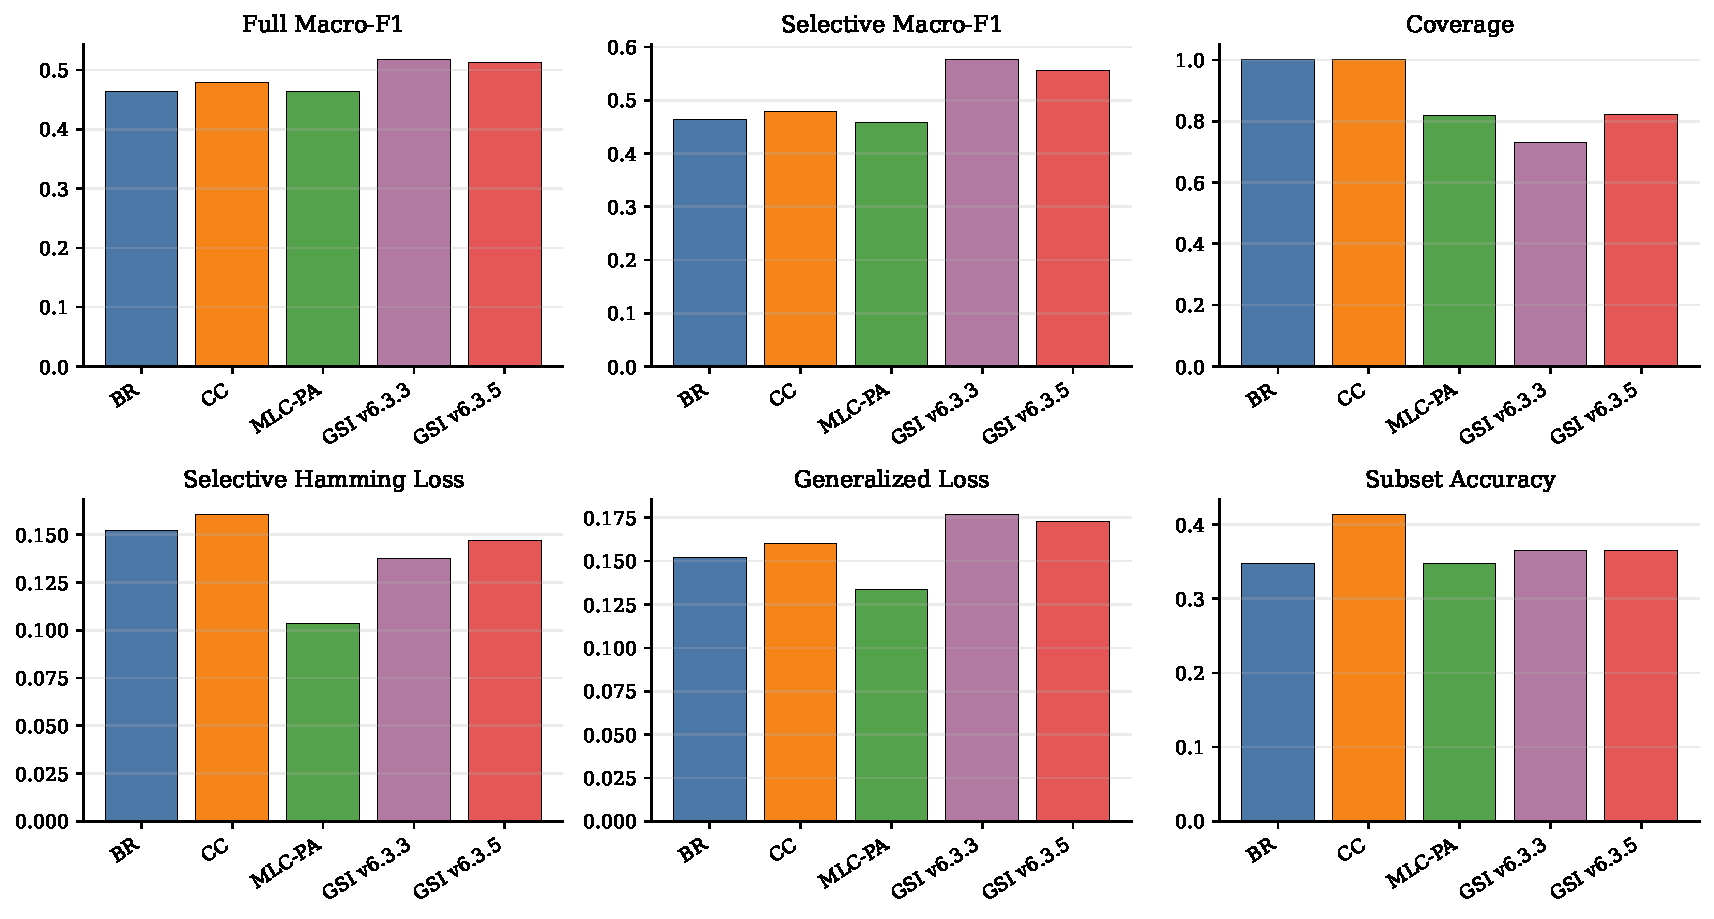
\includegraphics[width=\textwidth]{fig3_overall_metrics.pdf}
\caption{So sánh các metric trung bình. Với Hamming và generalized loss, giá trị thấp hơn tốt hơn.}\label{fig:overall}\end{figure}
\subsection{Kết quả theo từng tập dữ liệu}
\begin{table}[H]
\centering
\caption{Selective Macro-F1 trên từng tập dữ liệu.}
\label{tab:dataset-f1}
\small
\begin{tabular}{lccccc}
\toprule
Tập dữ liệu & BR & CC & MLC-PA & GSI v6.3.3 & GSI v6.3.5 \\
\midrule
emotions & 0.5972 & 0.5932 & 0.6172 & \textbf{0.7492} & 0.7048 \\
scene & 0.6994 & 0.7234 & 0.7431 & \textbf{0.7968} & 0.7322 \\
yeast & 0.3748 & 0.4017 & 0.3585 & \textbf{0.4719} & 0.4591 \\
plantpseaac & 0.1410 & 0.1715 & 0.0975 & \textbf{0.2684} & \textbf{0.2684} \\
humanpseaac & 0.1124 & 0.1397 & 0.0869 & \textbf{0.2377} & \textbf{0.2377} \\
chd49 & 0.5103 & 0.5073 & 0.5242 & 0.5140 & \textbf{0.5518} \\
music & 0.6067 & 0.6031 & 0.6375 & \textbf{0.7576} & 0.7217 \\
gpositivepseaac & 0.5535 & 0.5791 & 0.5370 & \textbf{0.6940} & 0.6425 \\
genbase & 0.6782 & 0.6930 & 0.6334 & \textbf{0.7700} & 0.7675 \\
viruspseaac & 0.3692 & 0.3836 & 0.3543 & \textbf{0.4994} & 0.4746 \\
\midrule
Trung bình & 0.4643 & 0.4796 & 0.4590 & \textbf{0.5759} & 0.5560 \\
\bottomrule
\end{tabular}
\end{table}
\begin{table}[H]
\centering
\caption{Coverage trên từng tập dữ liệu; giá trị lớn không tự thân đồng nghĩa chất lượng tốt hơn.}
\label{tab:dataset-coverage}
\small
\begin{tabular}{lccccc}
\toprule
Tập dữ liệu & BR & CC & MLC-PA & GSI v6.3.3 & GSI v6.3.5 \\
\midrule
emotions & \textbf{1.0000} & \textbf{1.0000} & 0.6749 & 0.7431 & 0.8884 \\
scene & \textbf{1.0000} & \textbf{1.0000} & 0.8871 & 0.7535 & 0.9805 \\
yeast & \textbf{1.0000} & \textbf{1.0000} & 0.7563 & 0.6359 & 0.7557 \\
plantpseaac & \textbf{1.0000} & \textbf{1.0000} & 0.9295 & 0.6826 & 0.6826 \\
humanpseaac & \textbf{1.0000} & \textbf{1.0000} & 0.9224 & 0.7021 & 0.7021 \\
chd49 & \textbf{1.0000} & \textbf{1.0000} & 0.6304 & 0.6202 & 0.7754 \\
music & \textbf{1.0000} & \textbf{1.0000} & 0.6887 & 0.7298 & 0.8573 \\
gpositivepseaac & \textbf{1.0000} & \textbf{1.0000} & 0.8584 & 0.7400 & 0.8536 \\
genbase & \textbf{1.0000} & \textbf{1.0000} & 0.9976 & 0.9414 & 0.9501 \\
viruspseaac & \textbf{1.0000} & \textbf{1.0000} & 0.8434 & 0.7690 & 0.7665 \\
\midrule
Trung bình & \textbf{1.0000} & \textbf{1.0000} & 0.8189 & 0.7318 & 0.8212 \\
\bottomrule
\end{tabular}
\end{table}
\begin{figure}[H]\centering
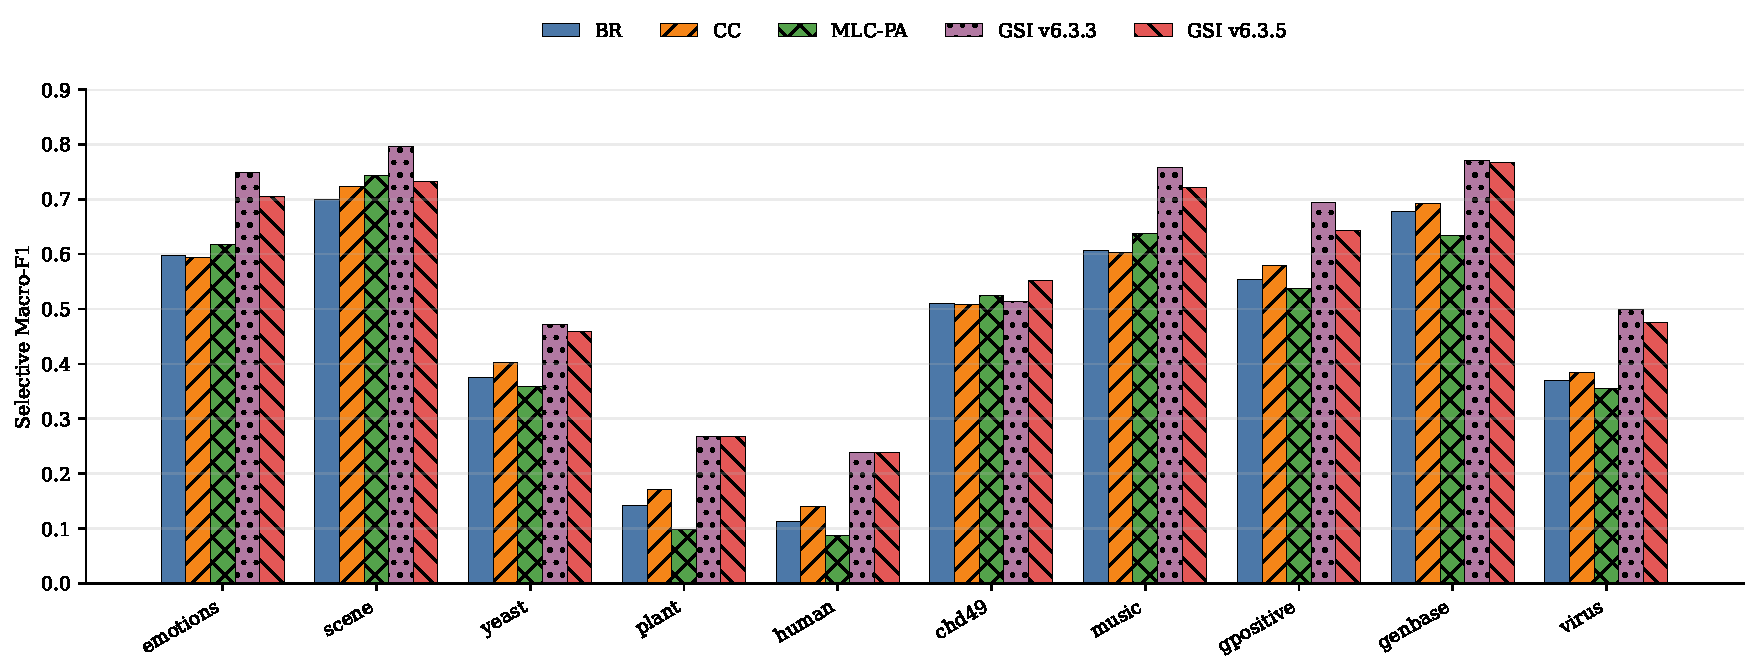
\includegraphics[width=\textwidth]{fig1_selective_macro_f1.pdf}
\caption{Selective Macro-F1 theo tập dữ liệu.}\label{fig:dataset-f1}\end{figure}
\begin{figure}[H]\centering
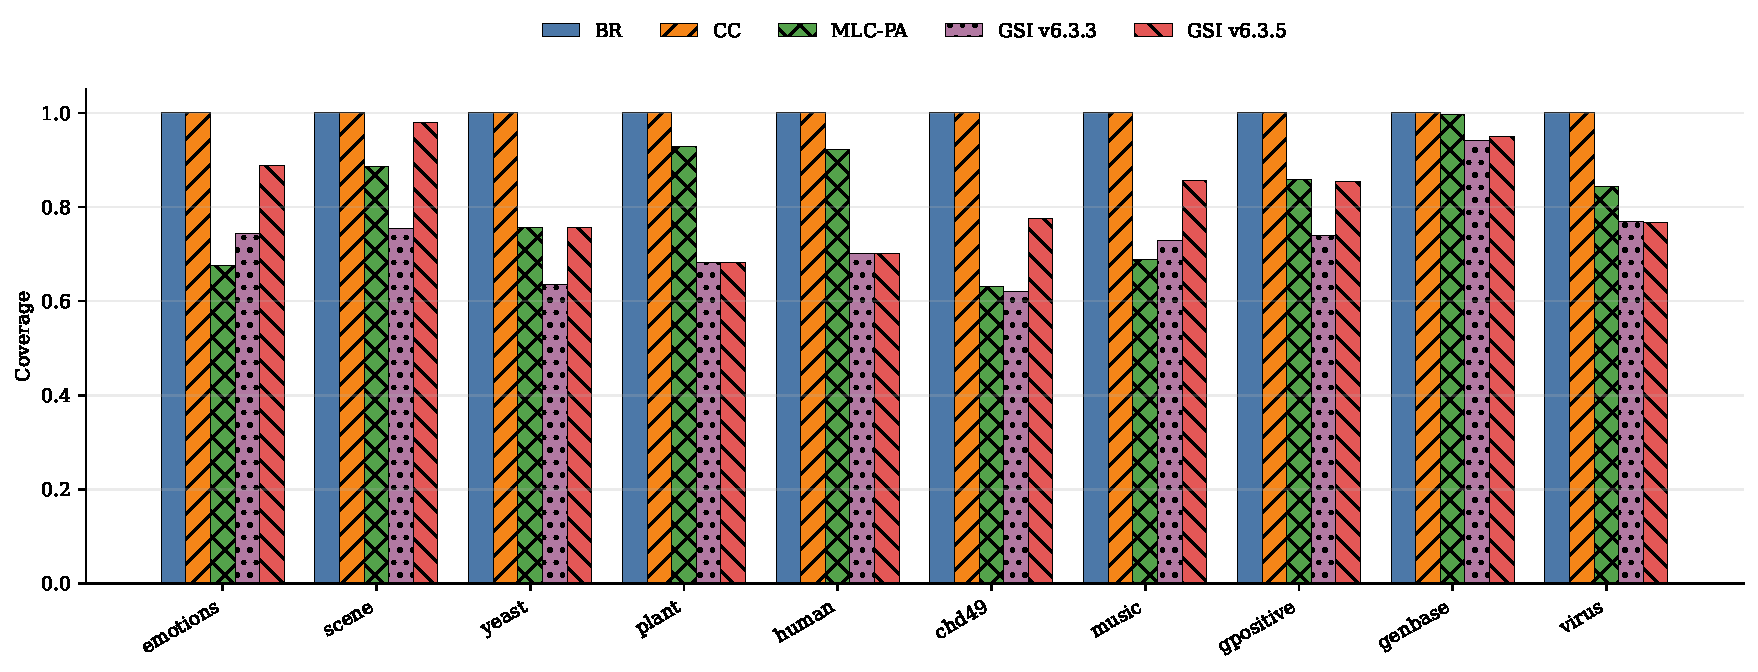
\includegraphics[width=\textwidth]{fig2_coverage.pdf}
\caption{Coverage theo tập dữ liệu. BR và CC luôn quyết định đầy đủ.}\label{fig:coverage}\end{figure}
Trên chd49, v6.3.5 tăng Selective Macro-F1 từ 0.5140 lên 0.5518 và coverage từ 0.6202 lên 0.7754. Tuy nhiên, audit theo nhãn cho thấy nhãn hiếm dương số 3 vẫn thuộc DL và F1 dương vẫn bằng 0; cải thiện toàn tập đến từ IL. Ngược lại, emotions, scene, music và gpositivepseaac giảm F1 khi các trường hợp IL khó bị buộc phải quyết định.
\subsection{Đánh đổi coverage--chất lượng}
\begin{figure}[H]\centering
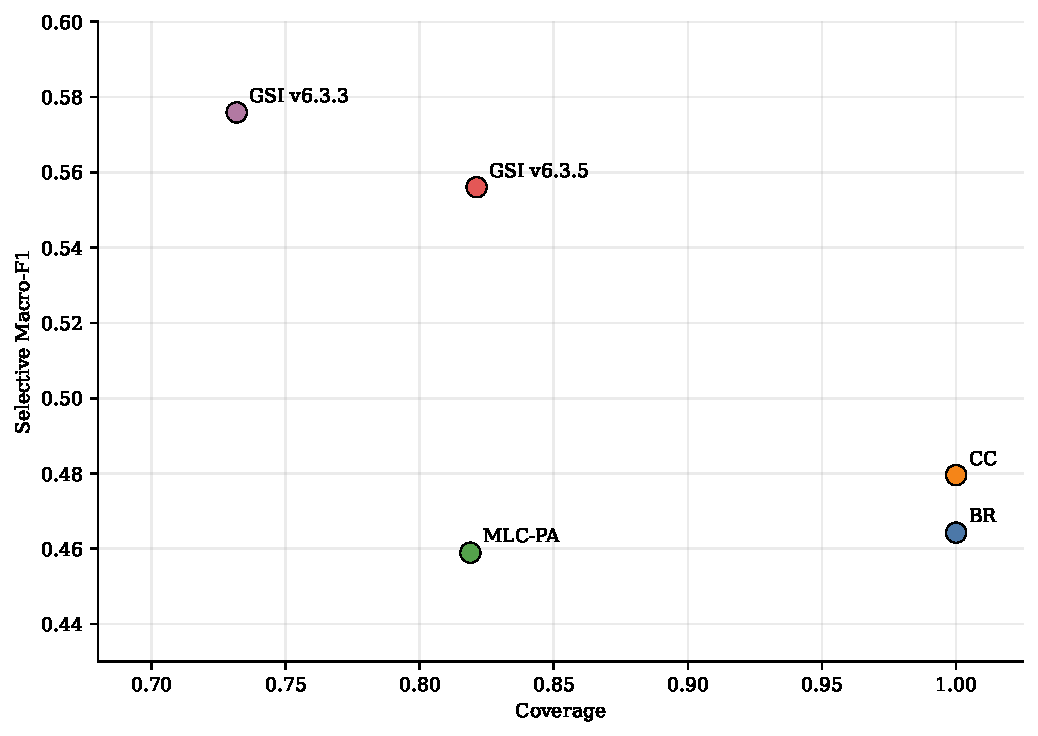
\includegraphics[width=0.78\textwidth]{fig4_f1_coverage_pareto.pdf}
\caption{Vị trí trung bình trên mặt phẳng coverage--Selective Macro-F1.}\label{fig:pareto}\end{figure}
\begin{figure}[H]\centering
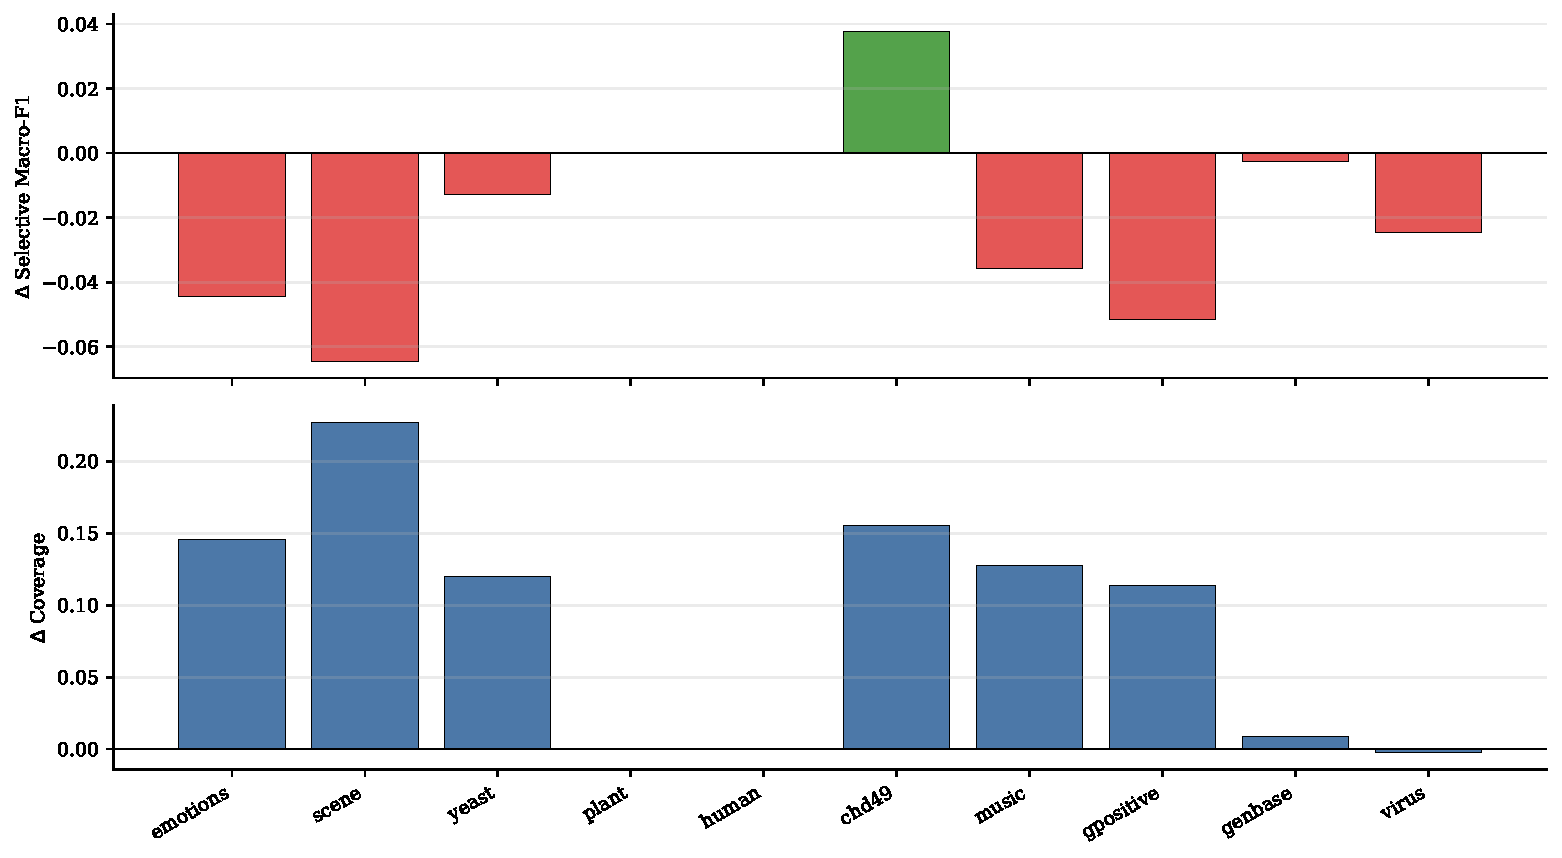
\includegraphics[width=0.92\textwidth]{fig5_v635_delta.pdf}
\caption{Chênh lệch v6.3.5 trừ v6.3.3 theo tập dữ liệu.}\label{fig:delta}\end{figure}
v6.3.5 nằm gần MLC-PA về coverage nhưng đạt Selective Macro-F1 cao hơn. v6.3.3 ưu tiên chất lượng dương trên vùng đã quyết định, trong khi v6.3.5 giảm tải từ chối cho IL. Lựa chọn giữa hai phiên bản vì vậy phụ thuộc chi phí review thực tế; chỉ nhìn F1 hoặc chỉ nhìn coverage đều không đủ.
\subsection{F1 dương, F1 âm và chất lượng vùng từ chối}
\begin{table}[H]
\centering
\caption{Chỉ số theo lớp và chất lượng vùng từ chối. RER không xác định đối với mô hình không từ chối.}
\label{tab:class-reject}
\scriptsize
\setlength{\tabcolsep}{3.5pt}
\resizebox{\textwidth}{!}{%
\begin{tabular}{lcccccc}
\toprule
Mô hình & $F_1^+$ & $F_1^-$ & Cov$^+$ & Cov$^-$ & ECR & RER \\
\midrule
BR & 0.4643 $\pm$ 0.2094 & 0.8688 $\pm$ 0.1104 & \textbf{1.0000 $\pm$ 0.0000} & \textbf{1.0000 $\pm$ 0.0000} & 0.0000 $\pm$ 0.0000 & -- \\
CC & 0.4796 $\pm$ 0.2026 & 0.8611 $\pm$ 0.1101 & \textbf{1.0000 $\pm$ 0.0000} & \textbf{1.0000 $\pm$ 0.0000} & 0.0000 $\pm$ 0.0000 & -- \\
MLC-PA & 0.4590 $\pm$ 0.2282 & \textbf{0.8944 $\pm$ 0.1121} & 0.6631 $\pm$ 0.1389 & 0.8641 $\pm$ 0.1007 & \textbf{0.4448 $\pm$ 0.1038} & \textbf{0.3949 $\pm$ 0.0561} \\
GSI v6.3.3 & \textbf{0.5759 $\pm$ 0.2089} & 0.8721 $\pm$ 0.1062 & 0.6978 $\pm$ 0.1467 & 0.7383 $\pm$ 0.0820 & 0.3815 $\pm$ 0.0397 & 0.2034 $\pm$ 0.0972 \\
GSI v6.3.5 & 0.5560 $\pm$ 0.1923 & 0.8635 $\pm$ 0.1150 & 0.8066 $\pm$ 0.1746 & 0.8152 $\pm$ 0.0991 & 0.2442 $\pm$ 0.1288 & 0.1926 $\pm$ 0.0957 \\
\bottomrule
\end{tabular}%
}
\end{table}
\begin{figure}[H]\centering
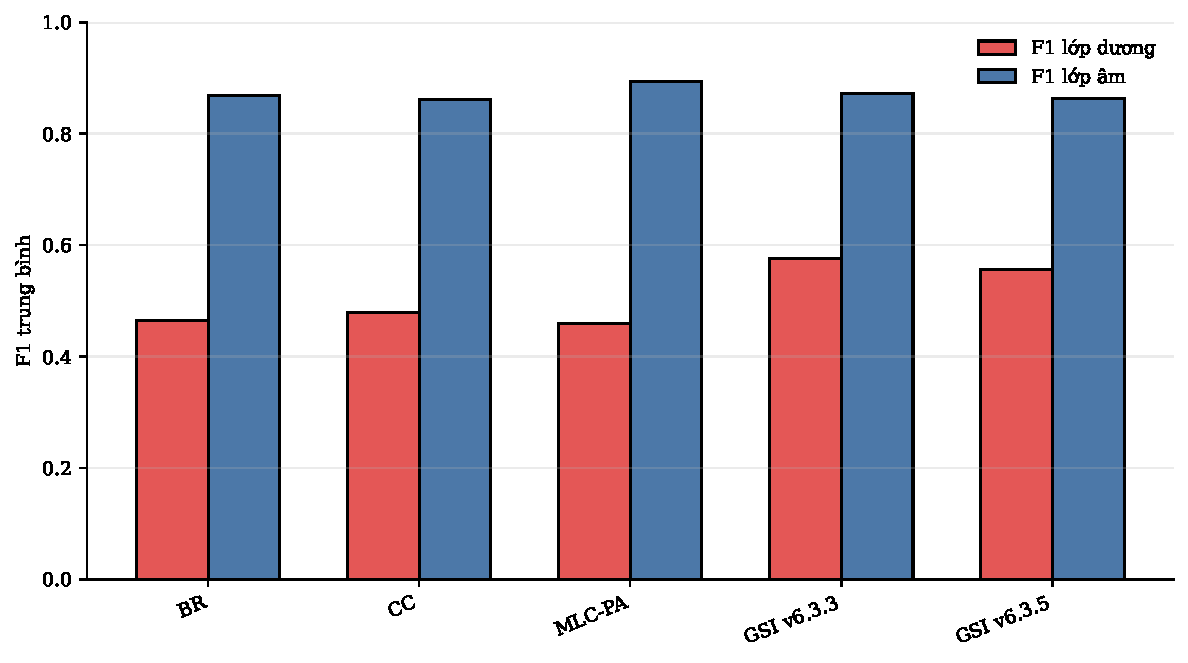
\includegraphics[width=0.82\textwidth]{fig6_positive_negative_f1.pdf}
\caption{Khoảng cách giữa F1 dương và F1 âm. F1 âm cao trên dữ liệu thưa có thể chủ yếu phản ánh prior lớp âm.}\label{fig:class-f1}\end{figure}
\begin{figure}[H]\centering
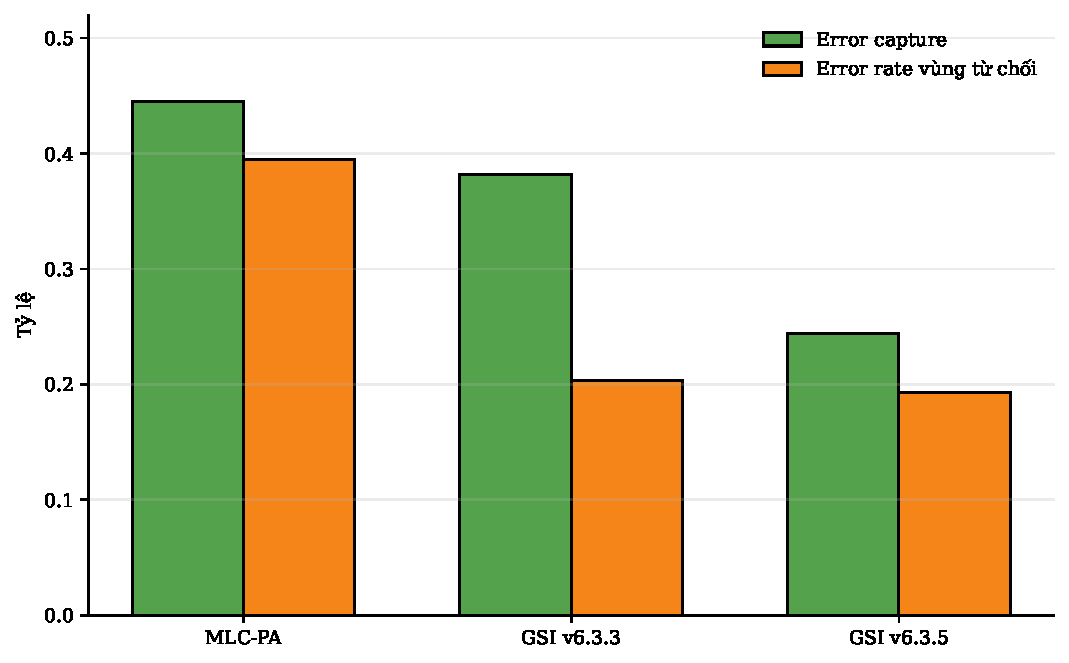
\includegraphics[width=0.72\textwidth]{fig7_rejection_quality.pdf}
\caption{Khả năng đưa lỗi full prediction vào vùng từ chối.}\label{fig:rejection}\end{figure}
Mọi mô hình đều có $F_1^-$ cao hơn $F_1^+$, đặc biệt trên dữ liệu thưa. Đây không phải bằng chứng rằng mô hình học tốt lớp thiểu số: một bộ phân loại thiên về 0 có thể đạt F1 âm rất cao. MLC-PA có ECR và RER cao nhất, nghĩa là vùng từ chối tập trung nhiều lỗi full prediction hơn; v6.3.3/v6.3.5 đổi một phần hiệu quả này lấy F1 dương cao hơn.
\subsection{Kiểm định thống kê}
Kiểm định Friedman trên Selective Macro-F1 trung bình của 10 tập cho kết quả $\chi^2=27.475$, $p=1.59e-05$, bác bỏ giả thuyết các mô hình có thứ hạng như nhau. Wilcoxon được thực hiện trên 10 giá trị trung bình theo dataset và hiệu chỉnh Holm; các fold không được coi là mẫu độc lập.
\begin{table}[H]
\centering
\caption{So sánh Wilcoxon ghép cặp ở mức tập dữ liệu: v6.3.5 trừ mô hình đối chứng. Giá trị $p$ được hiệu chỉnh Holm.}
\label{tab:wilcoxon}
\small
\begin{tabular}{lrrrrrr}
\toprule
Đối chứng & $\overline{\Delta F_1}$ & Thắng & Hòa & Thua & $W$ & $p_{Holm}$ \\
\midrule
BR & +0.0918 & 10 & 0 & 0 & 0.0 & 0.0078 \\
CC & +0.0765 & 10 & 0 & 0 & 0.0 & 0.0078 \\
MLC-PA & +0.0971 & 9 & 0 & 1 & 1.0 & 0.0078 \\
GSI v6.3.3 & -0.0199 & 1 & 2 & 7 & 5.0 & 0.0781 \\
\bottomrule
\end{tabular}
\end{table}
\noindent Thứ hạng trung bình Selective Macro-F1 (nhỏ hơn là tốt hơn): BR=4.10, CC=3.70, MLC-PA=4.00, GSI v6.3.3=1.30, GSI v6.3.5=1.90.
v6.3.5 cao hơn BR, CC và MLC-PA với $p_{Holm}<0.05$. Chênh lệch v6.3.5--v6.3.3 không đạt ý nghĩa ở mức 0.05; vì vậy không đủ bằng chứng thống kê để tuyên bố v6.3.3 vượt v6.3.5 về Selective Macro-F1 trên quần thể dataset, dù trung bình quan sát của v6.3.3 cao hơn.
\section{Thảo luận và giới hạn}
\begin{enumerate}
\item Báo cáo chỉ dùng Logistic Regression. Kết luận không tự động mở rộng sang SVM hoặc MLP.
\item Chỉ có 10 dataset; kiểm định thống kê có công suất hạn chế. Dataset, không phải fold, được dùng làm đơn vị kiểm định.
\item BR/CC có coverage 1 nên selective metric bằng full metric; so sánh trực tiếp với mô hình từ chối phải luôn xét đồng thời coverage hoặc generalized loss.
\item v6.3.5 đồng thời kế thừa SAMG2 của v6.3.4 và thay đổi phạm vi từ chối. Do đó chênh lệch v6.3.3--v6.3.5 không phải ablation đơn yếu tố hoàn toàn; ảnh hưởng thuần của phạm vi từ chối được kiểm tra bằng việc DL prediction giữ nguyên trong v6.3.5 so với v6.3.4.
\item F1 của nhãn cực hiếm có phương sai lớn. chd49 nhãn 3 chỉ có 16 mẫu dương; kết quả F1 bằng 0 phản ánh thiếu tín hiệu xếp hạng, không thể giải quyết chỉ bằng thay đổi phạm vi từ chối.
\item Thời gian fit được ghi nhận để audit nhưng không dùng kết luận tốc độ do benchmark chạy tuần tự trên một môi trường Windows không cô lập tải nền.
\end{enumerate}
\section{Kết luận}
v6.3.3 là lựa chọn tốt hơn khi ưu tiên Selective Macro-F1; v6.3.5 phù hợp hơn khi yêu cầu IL luôn có kết quả và coverage cao hơn. v6.3.5 không nên thay mặc định v6.3.3 chỉ dựa trên thử nghiệm hiện tại. Cách triển khai hợp lý là giữ \texttt{rejection\_scope=all\_labels} làm mặc định và cung cấp \texttt{dl\_only} như một operating mode có đánh đổi được mô tả rõ.
\appendix
\section{Ma trận kết quả đầy đủ}
Các bảng sau chứa trung bình 5 fold cho mọi metric được dùng trong báo cáo. Ký hiệu: MaF1/MiF1/ExF1 là full Macro/Micro/Example-F1; S là selective; GL là generalized loss; ECR là error-capture rate; RER là rejected-region error rate.
\begin{landscape}
\begin{longtable}{llrrrrr}
\caption{Các metric dự đoán đầy đủ theo từng tập dữ liệu và mô hình.}\label{tab:appendix-1}\\
\toprule
Dataset & Model & MaF1 & MiF1 & ExF1 & SubAcc & HL \\
\midrule
\endfirsthead
\toprule
Dataset & Model & MaF1 & MiF1 & ExF1 & SubAcc & HL \\
\midrule
\endhead
emotions & BR & 0.5972 & 0.6289 & 0.5455 & 0.2516 & 0.2013 \\
 & CC & 0.5932 & 0.6310 & 0.5957 & 0.2838 & 0.2240 \\
 & MLC-PA & 0.5972 & 0.6289 & 0.5455 & 0.2516 & 0.2013 \\
 & GSI v6.3.3 & 0.6733 & 0.6797 & 0.6386 & 0.2928 & 0.2030 \\
 & GSI v6.3.5 & 0.6733 & 0.6797 & 0.6386 & 0.2928 & 0.2030 \\
\addlinespace[2pt]
scene & BR & 0.6994 & 0.6938 & 0.6166 & 0.5361 & 0.0992 \\
 & CC & 0.7234 & 0.7110 & 0.7102 & 0.6623 & 0.1011 \\
 & MLC-PA & 0.6994 & 0.6938 & 0.6166 & 0.5361 & 0.0992 \\
 & GSI v6.3.3 & 0.7271 & 0.7172 & 0.7052 & 0.5514 & 0.1066 \\
 & GSI v6.3.5 & 0.7271 & 0.7172 & 0.7052 & 0.5514 & 0.1066 \\
\addlinespace[2pt]
yeast & BR & 0.3748 & 0.6351 & 0.6092 & 0.1465 & 0.2019 \\
 & CC & 0.4017 & 0.6198 & 0.5856 & 0.2019 & 0.2155 \\
 & MLC-PA & 0.3748 & 0.6351 & 0.6092 & 0.1465 & 0.2019 \\
 & GSI v6.3.3 & 0.4029 & 0.6366 & 0.6136 & 0.1490 & 0.2088 \\
 & GSI v6.3.5 & 0.4029 & 0.6366 & 0.6136 & 0.1490 & 0.2088 \\
\addlinespace[2pt]
plantpseaac & BR & 0.1410 & 0.2604 & 0.1848 & 0.1553 & 0.0945 \\
 & CC & 0.1715 & 0.3265 & 0.2725 & 0.2433 & 0.0988 \\
 & MLC-PA & 0.1410 & 0.2604 & 0.1848 & 0.1553 & 0.0945 \\
 & GSI v6.3.3 & 0.2003 & 0.2985 & 0.2203 & 0.1522 & 0.1016 \\
 & GSI v6.3.5 & 0.2003 & 0.2985 & 0.2203 & 0.1522 & 0.1016 \\
\addlinespace[2pt]
humanpseaac & BR & 0.1124 & 0.2851 & 0.2057 & 0.1526 & 0.0860 \\
 & CC & 0.1397 & 0.3774 & 0.3686 & 0.2929 & 0.0979 \\
 & MLC-PA & 0.1124 & 0.2851 & 0.2057 & 0.1526 & 0.0860 \\
 & GSI v6.3.3 & 0.1740 & 0.3423 & 0.2748 & 0.1880 & 0.0914 \\
 & GSI v6.3.5 & 0.1740 & 0.3423 & 0.2748 & 0.1880 & 0.0914 \\
\addlinespace[2pt]
chd49 & BR & 0.5103 & 0.6604 & 0.6349 & 0.1585 & 0.2940 \\
 & CC & 0.5073 & 0.6575 & 0.6333 & 0.1873 & 0.3009 \\
 & MLC-PA & 0.5103 & 0.6604 & 0.6349 & 0.1585 & 0.2940 \\
 & GSI v6.3.3 & 0.5039 & 0.6659 & 0.6431 & 0.1622 & 0.2929 \\
 & GSI v6.3.5 & 0.5039 & 0.6659 & 0.6431 & 0.1622 & 0.2929 \\
\addlinespace[2pt]
music & BR & 0.6067 & 0.6436 & 0.5695 & 0.2603 & 0.1957 \\
 & CC & 0.6031 & 0.6440 & 0.6104 & 0.2837 & 0.2165 \\
 & MLC-PA & 0.6067 & 0.6436 & 0.5695 & 0.2603 & 0.1957 \\
 & GSI v6.3.3 & 0.6772 & 0.6878 & 0.6448 & 0.3040 & 0.1952 \\
 & GSI v6.3.5 & 0.6772 & 0.6878 & 0.6448 & 0.3040 & 0.1952 \\
\addlinespace[2pt]
gpositivepseaac & BR & 0.5535 & 0.6865 & 0.6249 & 0.5954 & 0.1460 \\
 & CC & 0.5791 & 0.7127 & 0.7122 & 0.7032 & 0.1446 \\
 & MLC-PA & 0.5535 & 0.6865 & 0.6249 & 0.5954 & 0.1460 \\
 & GSI v6.3.3 & 0.6130 & 0.7054 & 0.6786 & 0.6184 & 0.1479 \\
 & GSI v6.3.5 & 0.6019 & 0.7057 & 0.6779 & 0.6204 & 0.1474 \\
\addlinespace[2pt]
genbase & BR & 0.6782 & 0.9797 & 0.9774 & 0.9547 & 0.0018 \\
 & CC & 0.6930 & 0.9809 & 0.9780 & 0.9577 & 0.0017 \\
 & MLC-PA & 0.6782 & 0.9797 & 0.9774 & 0.9547 & 0.0018 \\
 & GSI v6.3.3 & 0.7675 & 0.9885 & 0.9893 & 0.9743 & 0.0011 \\
 & GSI v6.3.5 & 0.7675 & 0.9885 & 0.9893 & 0.9743 & 0.0011 \\
\addlinespace[2pt]
viruspseaac & BR & 0.3692 & 0.4070 & 0.3411 & 0.2597 & 0.1995 \\
 & CC & 0.3836 & 0.4426 & 0.4049 & 0.3130 & 0.2025 \\
 & MLC-PA & 0.3692 & 0.4070 & 0.3411 & 0.2597 & 0.1995 \\
 & GSI v6.3.3 & 0.4321 & 0.4164 & 0.3644 & 0.2543 & 0.2079 \\
 & GSI v6.3.5 & 0.4083 & 0.4062 & 0.3551 & 0.2543 & 0.2096 \\
\addlinespace[2pt]
\bottomrule
\end{longtable}
\end{landscape}
\begin{landscape}
\begin{longtable}{llrrrrrr}
\caption{Các metric dự đoán chọn lọc theo từng tập dữ liệu và mô hình.}\label{tab:appendix-2}\\
\toprule
Dataset & Model & SMaF1 & SMiF1 & SInsF1 & SHL & GL & Cov \\
\midrule
\endfirsthead
\toprule
Dataset & Model & SMaF1 & SMiF1 & SInsF1 & SHL & GL & Cov \\
\midrule
\endhead
emotions & BR & 0.5972 & 0.6289 & 0.5455 & 0.2013 & 0.2013 & 1.0000 \\
 & CC & 0.5932 & 0.6310 & 0.5957 & 0.2240 & 0.2240 & 1.0000 \\
 & MLC-PA & 0.6172 & 0.6946 & 0.6913 & 0.1159 & 0.1760 & 0.6749 \\
 & GSI v6.3.3 & 0.7492 & 0.7561 & 0.7000 & 0.1778 & 0.2093 & 0.7431 \\
 & GSI v6.3.5 & 0.7048 & 0.7109 & 0.6617 & 0.1974 & 0.2087 & 0.8884 \\
\addlinespace[2pt]
scene & BR & 0.6994 & 0.6938 & 0.6166 & 0.0992 & 0.0992 & 1.0000 \\
 & CC & 0.7234 & 0.7110 & 0.7102 & 0.1011 & 0.1011 & 1.0000 \\
 & MLC-PA & 0.7431 & 0.7612 & 0.7459 & 0.0607 & 0.0877 & 0.8871 \\
 & GSI v6.3.3 & 0.7968 & 0.7903 & 0.7784 & 0.0952 & 0.1457 & 0.7535 \\
 & GSI v6.3.5 & 0.7322 & 0.7233 & 0.7097 & 0.1054 & 0.1093 & 0.9805 \\
\addlinespace[2pt]
yeast & BR & 0.3748 & 0.6351 & 0.6092 & 0.2019 & 0.2019 & 1.0000 \\
 & CC & 0.4017 & 0.6198 & 0.5856 & 0.2155 & 0.2155 & 1.0000 \\
 & MLC-PA & 0.3585 & 0.6725 & 0.6153 & 0.1437 & 0.1818 & 0.7563 \\
 & GSI v6.3.3 & 0.4719 & 0.6731 & 0.6107 & 0.1872 & 0.2283 & 0.6359 \\
 & GSI v6.3.5 & 0.4591 & 0.6977 & 0.6613 & 0.2064 & 0.2293 & 0.7557 \\
\addlinespace[2pt]
plantpseaac & BR & 0.1410 & 0.2604 & 0.1848 & 0.0945 & 0.0945 & 1.0000 \\
 & CC & 0.1715 & 0.3265 & 0.2725 & 0.0988 & 0.0988 & 1.0000 \\
 & MLC-PA & 0.0975 & 0.2012 & 0.3317 & 0.0709 & 0.0870 & 0.9295 \\
 & GSI v6.3.3 & 0.2684 & 0.4302 & 0.5656 & 0.0840 & 0.1525 & 0.6826 \\
 & GSI v6.3.5 & 0.2684 & 0.4302 & 0.5656 & 0.0840 & 0.1525 & 0.6826 \\
\addlinespace[2pt]
humanpseaac & BR & 0.1124 & 0.2851 & 0.2057 & 0.0860 & 0.0860 & 1.0000 \\
 & CC & 0.1397 & 0.3774 & 0.3686 & 0.0979 & 0.0979 & 1.0000 \\
 & MLC-PA & 0.0869 & 0.1918 & 0.3978 & 0.0577 & 0.0765 & 0.9224 \\
 & GSI v6.3.3 & 0.2377 & 0.4727 & 0.5496 & 0.0755 & 0.1424 & 0.7021 \\
 & GSI v6.3.5 & 0.2377 & 0.4727 & 0.5496 & 0.0755 & 0.1424 & 0.7021 \\
\addlinespace[2pt]
chd49 & BR & 0.5103 & 0.6604 & 0.6349 & 0.2940 & 0.2940 & 1.0000 \\
 & CC & 0.5073 & 0.6575 & 0.6333 & 0.3009 & 0.3009 & 1.0000 \\
 & MLC-PA & 0.5242 & 0.7208 & 0.6835 & 0.2163 & 0.2472 & 0.6304 \\
 & GSI v6.3.3 & 0.5140 & 0.6587 & 0.6225 & 0.2817 & 0.2886 & 0.6202 \\
 & GSI v6.3.5 & 0.5518 & 0.7174 & 0.6909 & 0.2857 & 0.2890 & 0.7754 \\
\addlinespace[2pt]
music & BR & 0.6067 & 0.6436 & 0.5695 & 0.1957 & 0.1957 & 1.0000 \\
 & CC & 0.6031 & 0.6440 & 0.6104 & 0.2165 & 0.2165 & 1.0000 \\
 & MLC-PA & 0.6375 & 0.6956 & 0.6966 & 0.1192 & 0.1757 & 0.6887 \\
 & GSI v6.3.3 & 0.7576 & 0.7672 & 0.7185 & 0.1663 & 0.2025 & 0.7298 \\
 & GSI v6.3.5 & 0.7217 & 0.7302 & 0.6745 & 0.1853 & 0.2017 & 0.8573 \\
\addlinespace[2pt]
gpositivepseaac & BR & 0.5535 & 0.6865 & 0.6249 & 0.1460 & 0.1460 & 1.0000 \\
 & CC & 0.5791 & 0.7127 & 0.7122 & 0.1446 & 0.1446 & 1.0000 \\
 & MLC-PA & 0.5370 & 0.7420 & 0.7405 & 0.1004 & 0.1287 & 0.8584 \\
 & GSI v6.3.3 & 0.6940 & 0.7817 & 0.7614 & 0.1263 & 0.1715 & 0.7400 \\
 & GSI v6.3.5 & 0.6425 & 0.7361 & 0.7139 & 0.1489 & 0.1706 & 0.8536 \\
\addlinespace[2pt]
genbase & BR & 0.6782 & 0.9797 & 0.9774 & 0.0018 & 0.0018 & 1.0000 \\
 & CC & 0.6930 & 0.9809 & 0.9780 & 0.0017 & 0.0017 & 1.0000 \\
 & MLC-PA & 0.6334 & 0.9852 & 0.9854 & 0.0013 & 0.0020 & 0.9976 \\
 & GSI v6.3.3 & 0.7700 & 0.9927 & 0.9941 & 0.0007 & 0.0183 & 0.9414 \\
 & GSI v6.3.5 & 0.7675 & 0.9903 & 0.9909 & 0.0009 & 0.0159 & 0.9501 \\
\addlinespace[2pt]
viruspseaac & BR & 0.3692 & 0.4070 & 0.3411 & 0.1995 & 0.1995 & 1.0000 \\
 & CC & 0.3836 & 0.4426 & 0.4049 & 0.2025 & 0.2025 & 1.0000 \\
 & MLC-PA & 0.3543 & 0.4316 & 0.4790 & 0.1471 & 0.1712 & 0.8434 \\
 & GSI v6.3.3 & 0.4994 & 0.5157 & 0.5117 & 0.1808 & 0.2081 & 0.7690 \\
 & GSI v6.3.5 & 0.4746 & 0.5086 & 0.5024 & 0.1803 & 0.2080 & 0.7665 \\
\addlinespace[2pt]
\bottomrule
\end{longtable}
\end{landscape}
\begin{landscape}
\begin{longtable}{llrrrrrrr}
\caption{Các chỉ số lớp và chất lượng từ chối theo từng tập dữ liệu và mô hình.}\label{tab:appendix-3}\\
\toprule
Dataset & Model & F1+ & F1- & Cov+ & Cov- & ECR & RER & ABS \\
\midrule
\endfirsthead
\toprule
Dataset & Model & F1+ & F1- & Cov+ & Cov- & ECR & RER & ABS \\
\midrule
\endhead
emotions & BR & 0.5972 & 0.8584 & 1.0000 & 1.0000 & 0.0000 & -- & 0.0000 \\
 & CC & 0.5932 & 0.8348 & 1.0000 & 1.0000 & 0.0000 & -- & 0.0000 \\
 & MLC-PA & 0.6172 & 0.9244 & 0.4729 & 0.7669 & 0.6091 & 0.3771 & 0.9237 \\
 & GSI v6.3.3 & 0.7492 & 0.8567 & 0.7635 & 0.7345 & 0.3495 & 0.2768 & 0.7144 \\
 & GSI v6.3.5 & 0.7048 & 0.8439 & 0.9105 & 0.8788 & 0.1363 & 0.2574 & 0.5102 \\
\addlinespace[2pt]
scene & BR & 0.6994 & 0.9404 & 1.0000 & 1.0000 & 0.0000 & -- & 0.0000 \\
 & CC & 0.7234 & 0.9378 & 1.0000 & 1.0000 & 0.0000 & -- & 0.0000 \\
 & MLC-PA & 0.7431 & 0.9644 & 0.7087 & 0.9261 & 0.4576 & 0.4023 & 0.5317 \\
 & GSI v6.3.3 & 0.7968 & 0.9346 & 0.8054 & 0.7421 & 0.3276 & 0.1416 & 0.8121 \\
 & GSI v6.3.5 & 0.7322 & 0.9328 & 0.9826 & 0.9801 & 0.0295 & 0.1601 & 0.1006 \\
\addlinespace[2pt]
yeast & BR & 0.3748 & 0.7666 & 1.0000 & 1.0000 & 0.0000 & -- & 0.0000 \\
 & CC & 0.4017 & 0.7717 & 1.0000 & 1.0000 & 0.0000 & -- & 0.0000 \\
 & MLC-PA & 0.3585 & 0.7830 & 0.6270 & 0.8124 & 0.4615 & 0.3822 & 0.9387 \\
 & GSI v6.3.3 & 0.4719 & 0.7973 & 0.5937 & 0.6543 & 0.4299 & 0.2465 & 0.9578 \\
 & GSI v6.3.5 & 0.4591 & 0.7722 & 0.8238 & 0.7262 & 0.2527 & 0.2160 & 0.9255 \\
\addlinespace[2pt]
plantpseaac & BR & 0.1410 & 0.9456 & 1.0000 & 1.0000 & 0.0000 & -- & 0.0000 \\
 & CC & 0.1715 & 0.9420 & 1.0000 & 1.0000 & 0.0000 & -- & 0.0000 \\
 & MLC-PA & 0.0975 & 0.9572 & 0.7396 & 0.9484 & 0.3028 & 0.4072 & 0.6493 \\
 & GSI v6.3.3 & 0.2684 & 0.9458 & 0.5073 & 0.6999 & 0.4366 & 0.1395 & 0.9898 \\
 & GSI v6.3.5 & 0.2684 & 0.9458 & 0.5073 & 0.6999 & 0.4366 & 0.1395 & 0.9898 \\
\addlinespace[2pt]
humanpseaac & BR & 0.1124 & 0.9487 & 1.0000 & 1.0000 & 0.0000 & -- & 0.0000 \\
 & CC & 0.1397 & 0.9349 & 1.0000 & 1.0000 & 0.0000 & -- & 0.0000 \\
 & MLC-PA & 0.0869 & 0.9626 & 0.6447 & 0.9481 & 0.3809 & 0.4228 & 0.7585 \\
 & GSI v6.3.3 & 0.2377 & 0.9480 & 0.5468 & 0.7165 & 0.4203 & 0.1288 & 0.9900 \\
 & GSI v6.3.5 & 0.2377 & 0.9480 & 0.5468 & 0.7165 & 0.4203 & 0.1288 & 0.9900 \\
\addlinespace[2pt]
chd49 & BR & 0.5103 & 0.6159 & 1.0000 & 1.0000 & 0.0000 & -- & 0.0000 \\
 & CC & 0.5073 & 0.6126 & 1.0000 & 1.0000 & 0.0000 & -- & 0.0000 \\
 & MLC-PA & 0.5242 & 0.6241 & 0.5629 & 0.6816 & 0.5363 & 0.4273 & 0.9349 \\
 & GSI v6.3.3 & 0.5140 & 0.6213 & 0.5809 & 0.6495 & 0.4036 & 0.3115 & 0.9312 \\
 & GSI v6.3.5 & 0.5518 & 0.5952 & 0.8331 & 0.7319 & 0.2434 & 0.3165 & 0.8053 \\
\addlinespace[2pt]
music & BR & 0.6067 & 0.8620 & 1.0000 & 1.0000 & 0.0000 & -- & 0.0000 \\
 & CC & 0.6031 & 0.8403 & 1.0000 & 1.0000 & 0.0000 & -- & 0.0000 \\
 & MLC-PA & 0.6375 & 0.9225 & 0.4960 & 0.7758 & 0.5805 & 0.3642 & 0.8952 \\
 & GSI v6.3.3 & 0.7576 & 0.8659 & 0.7389 & 0.7256 & 0.3783 & 0.2734 & 0.7415 \\
 & GSI v6.3.5 & 0.7217 & 0.8530 & 0.8835 & 0.8454 & 0.1852 & 0.2522 & 0.5945 \\
\addlinespace[2pt]
gpositivepseaac & BR & 0.5535 & 0.8949 & 1.0000 & 1.0000 & 0.0000 & -- & 0.0000 \\
 & CC & 0.5791 & 0.8926 & 1.0000 & 1.0000 & 0.0000 & -- & 0.0000 \\
 & MLC-PA & 0.5370 & 0.9287 & 0.7400 & 0.8983 & 0.4110 & 0.4246 & 0.4470 \\
 & GSI v6.3.3 & 0.6940 & 0.9021 & 0.7745 & 0.7284 & 0.3666 & 0.2092 & 0.6357 \\
 & GSI v6.3.5 & 0.6425 & 0.8939 & 0.9178 & 0.8320 & 0.1412 & 0.1463 & 0.4757 \\
\addlinespace[2pt]
genbase & BR & 0.6782 & 0.9991 & 1.0000 & 1.0000 & 0.0000 & -- & 0.0000 \\
 & CC & 0.6930 & 0.9991 & 1.0000 & 1.0000 & 0.0000 & -- & 0.0000 \\
 & MLC-PA & 0.6334 & 0.9993 & 0.9518 & 0.9999 & 0.3327 & 0.2639 & 0.0544 \\
 & GSI v6.3.3 & 0.7700 & 0.9996 & 0.9915 & 0.9389 & 0.3714 & 0.0071 & 0.5648 \\
 & GSI v6.3.5 & 0.7675 & 0.9995 & 0.9964 & 0.9478 & 0.2571 & 0.0034 & 0.4848 \\
\addlinespace[2pt]
viruspseaac & BR & 0.3692 & 0.8562 & 1.0000 & 1.0000 & 0.0000 & -- & 0.0000 \\
 & CC & 0.3836 & 0.8457 & 1.0000 & 1.0000 & 0.0000 & -- & 0.0000 \\
 & MLC-PA & 0.3543 & 0.8783 & 0.6871 & 0.8840 & 0.3752 & 0.4776 & 0.6516 \\
 & GSI v6.3.3 & 0.4994 & 0.8498 & 0.6755 & 0.7933 & 0.3308 & 0.2992 & 0.7329 \\
 & GSI v6.3.5 & 0.4746 & 0.8503 & 0.6638 & 0.7933 & 0.3398 & 0.3059 & 0.7279 \\
\addlinespace[2pt]
\bottomrule
\end{longtable}
\end{landscape}
\section{Khả năng tái lập}
\begin{verbatim}
python scripts/run_paper_v6_3_5_benchmark.py
python scripts/generate_paper_v6_3_5_report.py
\end{verbatim}
Môi trường ghi nhận: Python 3.13.14; NumPy 2.3.4; pandas 2.3.3; scikit-learn 1.7.2; SciPy 1.16.3; Matplotlib 3.10.7. Base commit của repository: \texttt{3fba3ec}; các thay đổi v6.3.4/v6.3.5 thuộc working tree của thực nghiệm này.
\begin{thebibliography}{9}
\bibitem{nguyen2021} V.-L. Nguyen and E. Hüllermeier. Multilabel Classification with Partial Abstention: Bayes-Optimal Prediction under Label Independence. \textit{Journal of Artificial Intelligence Research}, 72:613--665, 2021.
\bibitem{read2011} J. Read, B. Pfahringer, G. Holmes, and E. Frank. Classifier Chains for Multi-label Classification. \textit{Machine Learning}, 85:333--359, 2011.
\bibitem{chow1970} C. K. Chow. On Optimum Recognition Error and Reject Tradeoff. \textit{IEEE Transactions on Information Theory}, 16(1):41--46, 1970.
\bibitem{sechidis2011} K. Sechidis, G. Tsoumakas, and I. Vlahavas. On the Stratification of Multi-label Data. In \textit{ECML PKDD}, 2011.
\end{thebibliography}
\end{document}